\documentclass[12pt]{article}
\usepackage{amsmath}
\usepackage[dvipdfm]{graphicx}
\usepackage{bmpsize}
\usepackage{color}
\usepackage{hyperref}
\usepackage{float}
\usepackage{verbatim}
\usepackage{alltt}
\author{andruiman, \href{maito: andruiman@gmail.com}{andruiman@gmail.com}\footnote{To support this work please use our asset in AE: 5841059555983208287}}
\title{Multibranch forging algorithms: tails switching effect and chain measures}
\newcommand{\begver}{\begin{alltt}\begin{footnotesize}}
\newcommand{\enver}{\end{footnotesize}\end{alltt}}

\begin{document}

\maketitle
\begin{abstract}
In this paper we provide approach and simulation results for different measures applied to the block chains and their effect on the tails switching 
effect. Several measures types are investigating in terms of their influence on the distribution of the tails switching length. We also
present the positive effect of the network classicalization by additional single-branch nodes. Also some valuable physical analogues
are specified.
\end{abstract}

\noindent
{\bf Keywords:} PoS crypto-currencies, forging, multibranch, chain measures, Nothing-at-Stake, simulation

\section{Pre-introduction}

We continue the series of papers on various aspects of Proof-of-Stake forging algorithms. We act as the Consensus Research 
Group \url{http://consensusresearch.org} and publish our updates both on the website and the Nxt forum \url{https://nxtforum.org/consensus-research/}.
We plan to concentrate on one result in each paper and update our status with at least one new paper or software upload every two weeks describing 
what we will have achieved. For the papers that need corrections or important changes we will update in the usual way,
issuing the next versions. 
 

\section{Introduction}

Recently we had presented the series of papers concerning the multibranch forging algorithm which could be implemented as an alternative
to the classical single-branch approach currently used in the Nxt. As we showed, multibranch forging advantages are (1) normalization of
the blocks intervals (2) resistance to the long range attack \footnote{In the definition given in our previous paper \url{https://github.com/ConsensusResearch/articles-papers/blob/master/multistrategy/multistrategy.pdf}} (3) $\sim 1.5x$ higher
rate of blocks generated in comparison with the single-branch algo. However the still open question is the resistance of the multibranch forging
to the so called Nothing-at-Stake attack (again refer to the definition at the previous paper). In this paper we investigate potential solutions 
to the N@S problem in the multibranch environment and also investigate some of the valuable properties. 

\section{Tails switching}

The main reason to the N@S attack to be potentially executed is the property of the "tails switching" that is within the long run an arbitrary 
chain could win the competition in terms of the block measure function, which is classically defined as $m_0(b) = M/(\texttt{baseTarget}\ b)$ with 
some big constant $M$. Actually tails could be very long which leads to history rewriting and attacks abilities. To demonstrate this, suggest 
a simple binary tree (even deterministic) with $0$ in the root and branching with $0$ and $1$ in the nodes. Let's define a measure
function as a sum of numbers along the chain (branch). After $n$ generations the only one chain has the maximum measure $n$, with the total chains 
number of  $2^n$. The number of chains with the measure $2n-1$ is obviously $n$ \-- those are the chains with only one zero in one of 
the $n$ positions. So with growing number $n$ of generations the number of sub-maximum chains is also growing and these chains could potentially 
have nothing common with the best chain. Any stochastic event, if we now let it to occur, can occasionally change the best chain and therefore 
rewrite the history. The basic idea of preventing this effect is very low probability of the correct choosing the winning chain for an attacker 
due to exponential growth of the total chains number. However this probability doesn't go to zero even if an attacker keeps only $m$ best 
chains, selectively forging to one or another depending on his strategy. Generally speaking it is rather difficult to influence on the 
tail switching with extremely small stake as to do this, an attacker should generate at least one block within the certain number of blocks 
which algorithmically fix the history. We will consider even worse case when it is allowed to rewrite arbitrary amount of blocks without 
trying to fix something by check points. 

The long tails switching effect is not positive not even because of the N@S but also because it influences on the fee distribution, 
leads to recalculating the state and seeds uncertainty and doubts. However much of doubts could be eliminated as we realize that for the 
honest system all the chains represent exactly the same (or very close) vision as the best chain (after confirmations) if we keep the 
mapping of unpublished transactions and chains. The transaction processing algorithm we will discuss separately and now return to 
the tails switching. Different approaches are presented to choose the best chain with more measures (more relevantly with the measures combination), 
and that approach can actually help. If another measure chooses another subset of chains with extremely small intersection with
the subset chosen by the basic measure then it is very unlikely that attacker could win both the games. However another measure could
potentially lead to new kinds of vulnerabilities and require additional study. We will not discuss such an approach in this paper as
there is a wide range of possibilities and we better dedicate a separate paper to alternative measures calculated together and combined.
In this paper we suggest some more or less simple modifications to the basic measure. 

To choose the best chain and avoid the long tails switches we offer just to increase the measure of the currently best chain. To give a 
natural example let's consider a quantum particle and its paths. It is well known that the total QM amplitude could be presented as 
the Feynman's path integral (see e.g. \url{http://hitoshi.berkeley.edu/221a/pathintegral.pdf}): 
$$
\int \mathcal{D}x(t)e^{iS[x(t)]/\hbar},
$$
where $S[x(t)]$ represent an action along the path $x(t)$. {\it ...the classical equation of motion comes out in a very simple way.
If you take the limit $\hbar\to 0$, the weight factor $e^{iS[x(t)]/\hbar}$ oscillates very rapidly. Therefore, we expect that the main
contribution to the path integral comes from paths that make the action stationary. This is nothing but the derivation of Euler-Lagrange 
equation from the classical action. Therefore, the classical trajectory dominates the path integral in the small $\hbar$ limit.}
So this allows to effectively "choose"\footnote{This choice is performed by the nature} the only one path minimizing the action along it in the
classical limit. 

We can do something similar. Let's modify the measure function with a factor depending on the current cumulative measure of the 
chain $m(b)=h(\texttt{cumulativeDifficulty} b') m_0(b)$ where $b'$ is the parent block and $\texttt{cumulativeDifficulty}$
is given by the sum of difficulties of the all precedent blocks. Along with the "smooth" function $h(\cdot)$ we can also introduce the direct 
factor which behaves like $\theta$-function with respect to the fact of being the last of the best chain for the parent block $b'$. We can define 
it like $(k(b') = {\rm if}\ ({\rm best}\ b')\ {\rm then}\ K\ {\rm else}\ 1)$ and redefine $m(b)=h(\texttt{cumulativeDifficulty\ b'}) k(b') m_0(b)$. 
This trick allows to save the multibranch algorithm with all its benefits but lets it converge faster. It should be noted that for different 
nodes the best chains can potentially be different at the moment and in the single-branch approach this could lead to the temporal network clustering 
but not in the multibranch case. The consensus procedure has to draws different "best" chains together leaving however short tails switching.
The simulating model presented below suggests immediate block propagation and we realize this restriction\footnote{At the moment of the paper issuing
we have already multibranching software with delayed propagation and we will present its results very soon}. If this approach works as designed we 
can introduce the number of confirmations (even calculate it) which fixes the history with some chosen probability.

Another interesting observation could be made if we add the single-branch nodes to the system. They work the same way as the tricky measure as they forge
only to the best chain. So classical nodes add classical behavior to this "quantum" process. This reflects the psi-function collapse effect as
{\it a measurement modifies the system}. Here the "measurement" is the the best chain choice, while branching is just a process. 

Below in this paper we will present the simulation results for all the cases with different measure functions and in the different environments.

Resuming we'd like to note that:
\begin{itemize}
\item[1.] {Multibranch approach reflects the quantum system behavior.}
\item[2.] {As long as we design the convergent system we need the paths weight factor.}
\item[3.] {Classical nodes behaves like measurements in QM choosing the best chain and collapsing the "wave" function.}
\item[4.] {We need to choose not extremely large factors to leave the multibranching effect as it secures the system.} 
\item[5.] {We expect deeper inspiration from the QM analogue in the further study.}
\end{itemize}

\section{Pure multibranch environment with smooth $h$ functions}

In this section we provide the results about the distribution of the tails switching length for the smooth $h$ functions given 
as a certain power of the $\texttt{ptd}/\texttt{btd}$ relation, where \texttt{ptd} is the current cumulative difficulty of the
chain determined by the last forging block and \texttt{btd} is the cumulative difficulty of the best chain. So we define
$m(b) = (\texttt{ptd}/\texttt{btd})^n m_0(b)$. Below we present the results with $n=1,2,4,8$. The network consists of
two equal accounts, \texttt{tfdepth} parameter is set to $200$, time of simulation is set to $T=15000$ ticks, $\tau=10$.
The distribution is given for numbers more than zero to save the axis scale.

\begin{figure}[H]
\centering
\caption{$n=0$ \-- no correction}
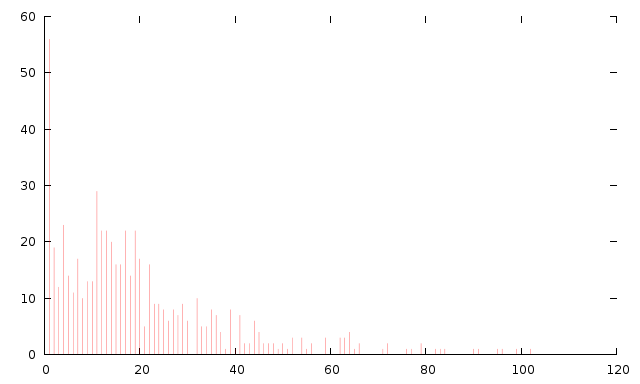
\includegraphics[scale=0.6]{changes-n0k1.png}
\end{figure} 

\begin{figure}[H]
\centering
\caption{$n=1$}
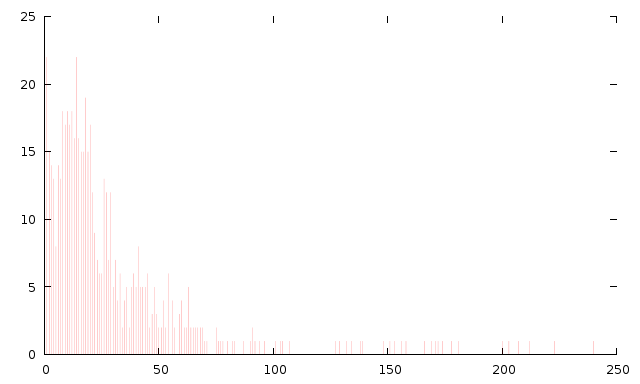
\includegraphics[scale=0.6]{changes-n1k1.png}
\end{figure} 

\begin{figure}[H]
\centering
\caption{$n=2$}
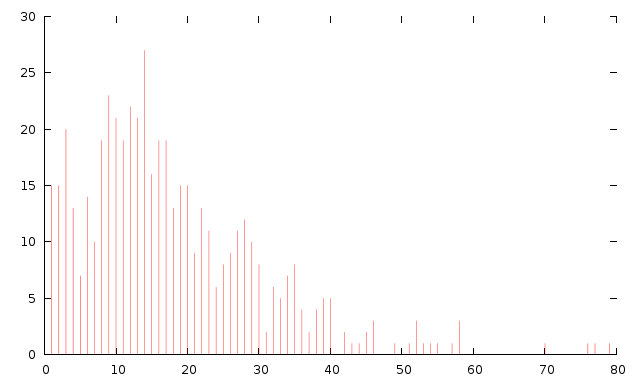
\includegraphics[scale=0.6]{changes-n2k1.png}
\end{figure} 

\begin{figure}[H]
\centering
\caption{$n=4$}
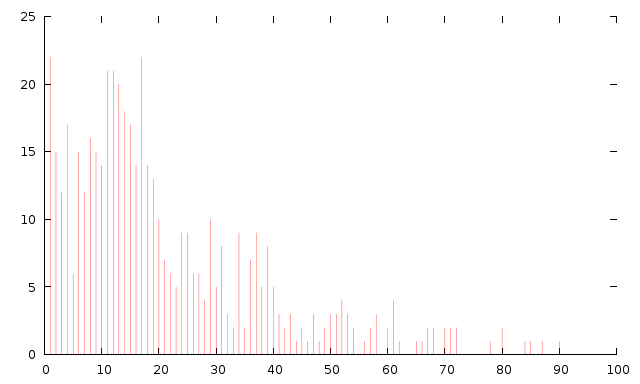
\includegraphics[scale=0.6]{changes-n4k1.png}
\end{figure} 

For the simulated distributions we are to conclude that there is not essential effects from the smooth $h$ functions to
preventing the long tails switches. This result shows that system consists of several chains with very close measure (even
maybe equal) and such measuring advances all of them. Also the small number of nodes (two) matters of course. In real network
there is much lower probability of equal chains (this effect can be also neglected by the timestamp measuring in smaller units).
We need now to investigate the direct procedure of advancing of the best chain. 

\section{Pure multibranch environment with the direct $k$ factor}

In this section we present the results for the same simulation environment but with different $k=2,4,6$ parameter and $n=0$.

\begin{figure}[H]
\centering
\caption{$k=2$}
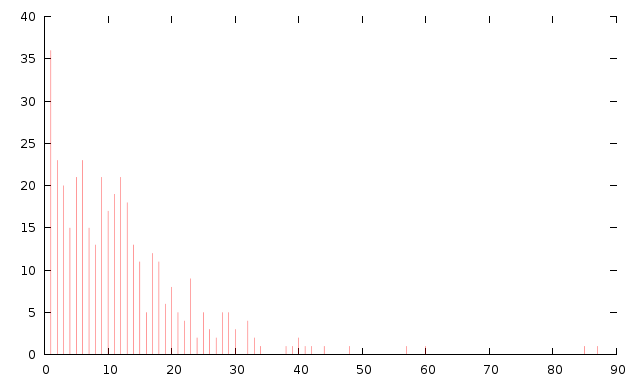
\includegraphics[scale=0.6]{changes-n0k2.png}
\end{figure} 

\begin{figure}[H]
\centering
\caption{$k=4$}
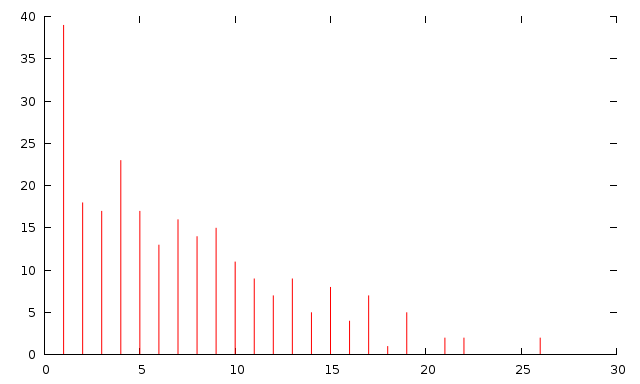
\includegraphics[scale=0.6]{changes-n0k4.png}
\end{figure} 

\begin{figure}[H]
\centering
\caption{$k=6$}
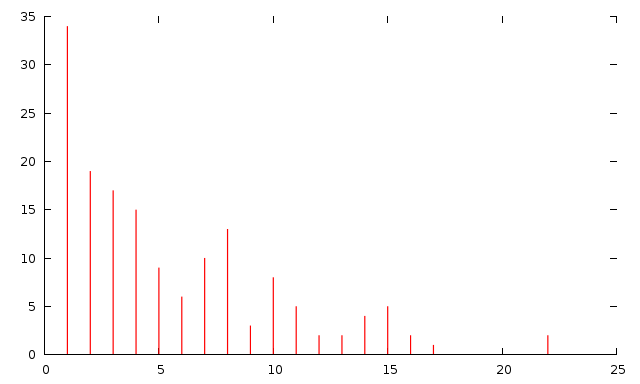
\includegraphics[scale=0.6]{changes-n0k6.png}
\end{figure} 

The direct factor for advancing the best chain works as we expected reducing the total number of switches and shortening the switching tails length.
Let's now observe what happens if we add some classical nodes. 

\section{Multibranch environment with "classicalization"}

Let's add a single-branch node to stabilize the measurements and set other stabilizing parameters to its default values $k=1,n=0$.
So the number of accounts is set to $N=2+1$ and we carry out the simulations for the cases of $5\%,10\%,20\%,50\%$ of the single-branch stake.

\begin{figure}[H]
\centering
\caption{Single-branch stake 5\%}
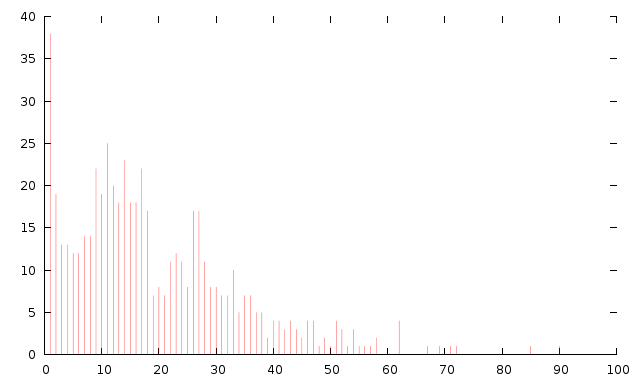
\includegraphics[scale=0.6]{changes-s5n0k1.png}
\end{figure} 

\begin{figure}[H]
\centering
\caption{Single-branch stake 10\%}
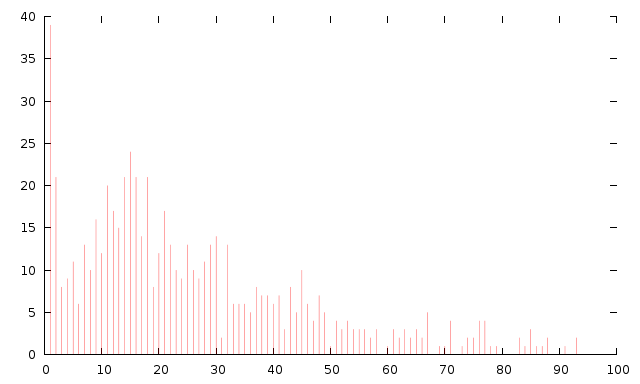
\includegraphics[scale=0.6]{changes-s10n0k1.png}
\end{figure} 

\begin{figure}[H]
\centering
\caption{Single-branch stake 20\%}
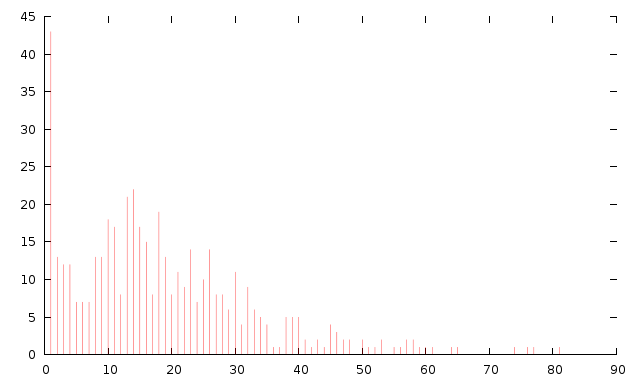
\includegraphics[scale=0.6]{changes-s20n0k1.png}
\end{figure} 

\begin{figure}[H]
\centering
\caption{Single-branch stake 50\%}
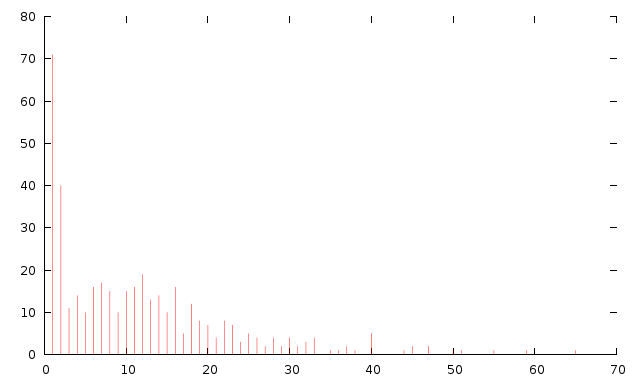
\includegraphics[scale=0.6]{changes-s50n0k1.png}
\end{figure} 

We can observe that the single-branch account advances the best chain propagating only for larger stake, but it works as predicted, shortening tails length
and reducing the total number of switches. Now we will mix all the methods.

\section{Methods combination}

\begin{figure}[H]
\centering
\caption{$n=2,k=2$}
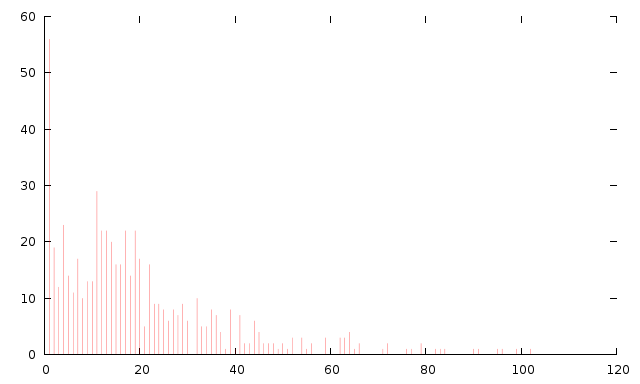
\includegraphics[scale=0.6]{changes-s0n2k2.png}
\end{figure} 

\begin{figure}[H]
\centering
\caption{$n=4,k=2$}
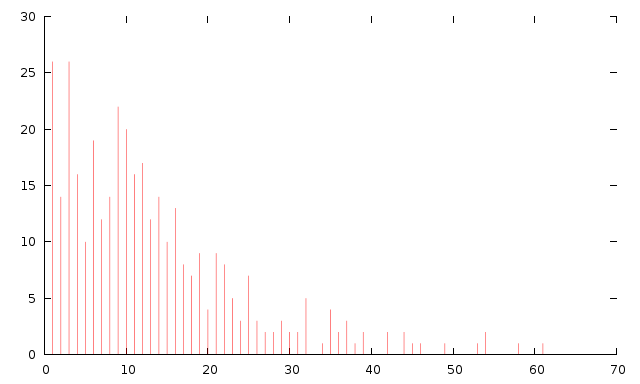
\includegraphics[scale=0.6]{changes-s0n4k2.png}
\end{figure} 

\begin{figure}[H]
\centering
\caption{$n=2,k=4$}
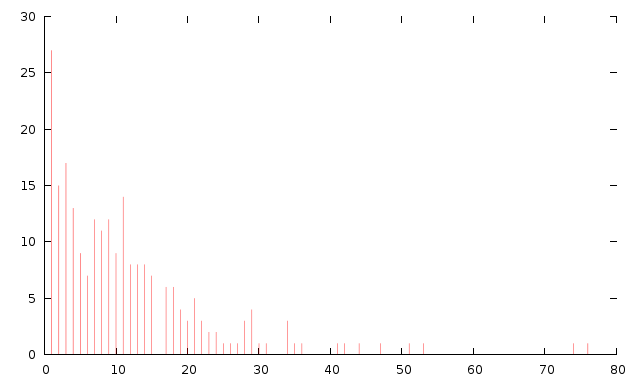
\includegraphics[scale=0.6]{changes-s0n2k4.png}
\end{figure} 

Here we present the distribution for the $8$-nodes system with 4 multibranch (80\% stake) and 4 single-branch (20\% stake) accounts and for 
a longer run.

\begin{figure}[H]
\centering
\caption{$N=4+4,n=2,k=4$, single-branch stake is 20\%, $T=25000$}
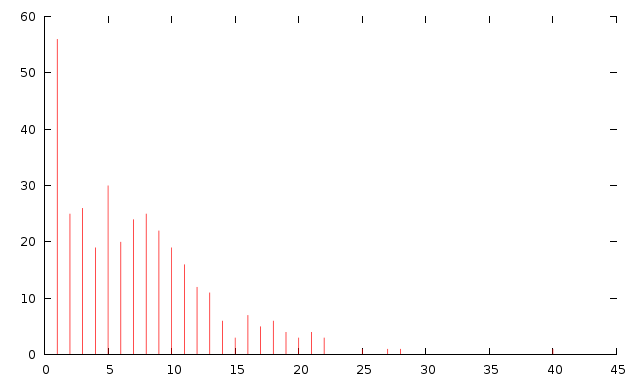
\includegraphics[scale=0.6]{changes-8s20n2k4.png}
\end{figure} 

\section{More physical inspirations}
Interesting simulations can be made with the following physical analogue. Suggest a classical particle in some special "fields" with
motion equations like following:
$$
\ddot x(t) = m\ u(t) + k\ x(t),\ \ddot x(t) = m\ u(t) + k\ \dot x(t),
$$
where the first equation reflects the additional force proportional to the current coordinate (like inverse tension with $k>0$) and the second
represent "inverse" viscosity effect with the force proportional to the velocity. Solving the simplified equations (with $u(t)\equiv 1)$, 
generalizing solutions and discretizing them we get the following recurrent expression:
$$
x_{n+1}=(1+kn^\alpha)x_n + m_{n+1}.
$$
We can interpret the values as $x_n$ for the cumulative measure of the chain, $m_n$ for the measure of the current block, $n$ for the block height (or timestamp),
$k,n,\alpha$ for regulating parameters.


\section{Conclusion and future work}
In this paper we provide simulation results for different measures applied to the block chains and their effect on the tails switching effect.
We observed that (1) smooth measure correcting works not perfect but its effect can be adequate for the larger network with small timestamp unit 
(2) the procedure of the direct increase of the best chain measure works as predicted (3) the network classicalization effect with additional 
single-branch nodes are demonstrated. We also provide some physical analogues which help to carry the future study out. It includes 
(1) study of convergence procedure in the network with delayed propagation (2) transaction processing algorithm study for the multibranch environment
(3) measures combinations effect investigation (4) study of the extended set of the smooth measures influence.

\end{document}




